\documentclass[11pt, a4paper]{article}

\usepackage[utf8]{inputenc}
\usepackage[T1]{fontenc}
\usepackage[english]{babel}
\usepackage{hyperref}
\usepackage{framed}
\usepackage{geometry}
\usepackage{tikz}
\usetikzlibrary{arrows,shapes,snakes,positioning}
\usepackage{lscape}
\usepackage{csquotes}

\title{LINGI2251: Assignment 1}
\author{Florian Thuin}
\date{\today}

\begin{document}
\maketitle
\tableofcontents

\section{Requirement issues and adopted corrections}

\paragraph{Requirement 1} After the purchase of gasoline, the gas pump
reports the number of gallons purchased to the GSCS.\@ The GSCS updates the
remaining inventory.

\paragraph{Requirement 2} After the purchase of gasoline, the gas pump
reports the dollar amount of the purchase to the GSCS.\@ The maximum value of
a purchase is $\$~999.99$. The GSCS then causes the gas pump interface to
query the customer as to payment type.

\begin{framed}
    \paragraph{Critics} 
    \begin{itemize}
        \item Requirement 1 and 2 are strongly connected because the
            amount of dollar depend of the number of gallons.

            In this way, we thinks that it will only be one
            requirement instead of two.

        \item "After" is a infinite length of time and must be more
            precise such as "Directly after".
    \end{itemize}

    \paragraph{Requirement 1 and 2} Directly after the purchase of gasoline,
    the gas pump reports the number of gallons purchased and the
    dollar amount of the purchase to the GSCS. The maximum value of
    a purchase is $\$999.99$. 
    When the GSCS receive the report, he updates the remaining
    inventory and cause the gas pump interface to query the customer as to
    payment type. 

\end{framed}

\paragraph{Requirement 3} The customer may choose to be billed at the time
of purchase, or to be sent a monthly bill. If billing is to be done at time
of purchase, the gas pump interface queries the customer as to whether
payment will be made by cash or credit card. If the purchase is to be placed
on a monthly bill, the gas pump interface instructs the customer to see the
cashier. If an invalid or no response is received, the GSCS bills at the
time of purchase.

\begin{framed}
    \paragraph{Critics} 
    \begin{itemize}
        \item There should be a time limit to says that there is no
            response.
        \item It's not explicit that the customer choose how to pays
            through gas pump interface.
    \end{itemize}

    \paragraph{Requirement 3} When the gas pump interface query the
    customer as to payment type, he may choose to be billed at the
    time of purchase, or to be sent a monthly bill. 
    If billing is to be done at time of purchase, the gas pump
    interface queries the customer as to whether payment will be
    made by cash or credit card. If the purchase is to be placed on
    a monthly bill, the gas pump interface instructs the customer to
    see the cashier. If an invalid response is receive or there is
    no response during one minute, the GSCS bills at the time of purchase.
\end{framed}

\paragraph{Requirement 4} If the customer has selected to pay at the time of
purchase, he or she can choose to pay by cash or credit card. If the
customer selects cash, the gas pump interface instructs the customer to see
the cashier. If the customer selects credit card, the gas pump interface
instructs the customer to swipe his or her credit card through the credit
card reader. If an invalid or no selection is made, the GSCS will default
to credit card payment.

\begin{framed}
    \paragraph{Critics} 
    \begin{itemize}
        \item There should be a time limit to says that there is no
            response.
    \end{itemize}

    \paragraph{Requirement 4} If the customer has selected to pay at the time of
    purchase, he or she can choose to pay by cash or credit card. If the
    customer selects cash, the gas pump interface instructs the customer to see
    the cashier. If the customer selects credit card, the gas pump interface
    instructs the customer to swipe his or her credit card through the credit
    card reader. If an invalid selection or no selection during one
    minute is made, the GSCS will default to credit card payment.
\end{framed}

\paragraph{Requirement 5} If payment is to be made by credit card, then the
card reader sends the credit card number to the GSCS.\@ If the GSCS receives
an invalid card number, then a message is sent to the gas pump interface
asking the customer to swipe the card through the card reader again. After
the account number is obtained, the account number and purchase price are
sent to the credit card system, and the GSCS and gas pump interface are
reset to their initial state. The purchase price sent can be up
to \${}10000.

\begin{framed}
    \paragraph{Critics} 
    \begin{itemize}
        \item It's not complete because the requirement don't take in
            account that potentially the card reader is not able to read
            the card for some extern reason such as a invalid card or a
            issues with the card reader.
        \item It's not consistent to have a purchase price up to \$10000
            because the requirement 2 says a upper bound to \$999.99.
    \end{itemize}

    \paragraph{Requirement 5} If payment is to be made by credit card, then the
    card reader sends the credit card number to the GSCS.\@ If the GSCS receives
    an invalid card number, then a message is sent to the gas pump interface
    asking the customer to swipe the card through the card reader again.
    If after three times the account is not obtained, the gas pump
    interface instructs the customer to see the cashier.
    If the account number is obtained within the three times, the
    account number and purchase price are
    sent to the credit card system, and the GSCS and gas pump interface are
    reset to their initial state. The purchase price sent can be up
    to \${}999.99.
\end{framed}

\paragraph{Requirement 6} The cashier is responsible for accepting the
customer's payment and making change, if necessary. When payment is
complete, the cashier indicates this on the cashier's interface. The GSCS
and the gas pump interface then return to the initial state.

\begin{framed}
    \paragraph{Critics} 
    \begin{itemize}
        \item The cashier is responsible for accepting cash payment or
            monthly billing but not credit card payment.
    \end{itemize}

    \paragraph{Requirement 6} The cashier is responsible for accepting
    monthly billing or the
    customer's cash payment and making change, if necessary. When payment is
    complete, the cashier indicates this on the cashier's interface. The GSCS
    and the gas pump interface then return to the initial state.
\end{framed}

\paragraph{Requirement 7} If payment is to be made by monthly bill, the
purchase price is displayed on the cashier's interface. The cashier
selects an option from the cashier's interface, alerting the GSCS that the
payment will be placed on a monthly bill. The GSCS then prompts the cashier
to enter the billing account number.

\paragraph{Requirement 8} The customer must give the billing account number
to the cashier, who then enters it at the cashier's interface. If a valid
billing account number is entered, then the billing account number, purchase
price, and a brief description of the type of transaction is logged. If an
invalid billing account number is entered, an error message is displayed
and the cashier is prompted to enter it again. The cashier must also have
the option to cancel the operation, in which case the cashier's interface
reverts to showing the purchase price and the cashier can again either
receive cash or indicate that monthly billing should be used.

\begin{framed}
    \paragraph{Critics} 
    \begin{itemize}
        \item There is no sens to have two different requirement mainly
            if the requirement 8 is more complete than the requirement
            7. Indeed, the requirement 7 don't take in account the
            case where the customer has no ability to perform a
            monthly billing.
    \end{itemize}

    \paragraph{Requirement 7 and 8} If payment is to be made by monthly bill, the
    purchase price is displayed on the cashier's interface.
    The customer must give the billing account number
    to the cashier, who then enters it at the cashier's interface. If a valid
    billing account number is entered, then the billing account number, purchase
    price, and a brief description of the type of transaction is logged. If an
    invalid billing account number is entered, an error message is displayed
    and the cashier is prompted to enter it again. The cashier must also have
    the option to cancel the operation, in which case the cashier's interface
    reverts to showing the purchase price and the cashier can again either
    receive cash or indicate that monthly billing should be used.
\end{framed}

\paragraph{Requirement 9} To pay a monthly bill, the customer must send
the payment along with the billing account number. The cashier enters
monthly payments by first selecting the appropriate option from the
cashier's interface. The GSCS then sends a message to the cashier's
interface. The GSCS then sends a message to the cashier's interface
prompting the cashier to enter the billing account number, the amount
remitted, and the type of payment. If any of these pieces of information
are not entered or are invalid, payment cannot be processed; an error
message will be displayed, and the cashier's interface will be returned
to the previous screen. If the type of payment is credit card, the credit
card account number must also be entered, and then the paper credit card
receipt will be photocopied and stored with the rest of the year's receipts.

\begin{framed}
    \paragraph{Critics} 
    \begin{itemize}
        \item It's ambiguous because we don't know how the customer send
            the payment. By mail or go to the gas pomp?

        \item "by selection the appropriate option" is not precise
            enough because the appropriate option is in fact "pay a
            monthly bill".

        \item The fact that the receipt will be photocopied is
            completely irrelevant for the system.
    \end{itemize}

    \paragraph{Requirement 9} To pay a monthly bill, the customer must send
    the payment along with the billing account number. The cashier enters
    monthly payments by first selecting the appropriate option from the
    cashier's interface. The GSCS then sends a message to the cashier's
    interface. The GSCS then sends a message to the cashier's interface
    prompting the cashier to enter the billing account number, the amount
    remitted, and the type of payment.
    If the type of payment is credit card, the credit
    card account number must also be entered.
    If any of these pieces of information
    are not entered or are invalid, payment cannot be processed; an error
    message will be displayed, and the cashier's interface will be returned
    to the previous screen. 
    If these pieces of informations are valid, then the transaction is logged.
\end{framed}

\paragraph{Requirement 10} Unless otherwise specified, if the GSCS receives
invalid input it will send an error message to the cashier's interface.
The cashier will be expected to take appropriate action, which may
involve shutting the system down for maintenance.

\begin{framed}
\end{framed}

\paragraph{Non-functional requirement 1} The system must always respond to
customer input within 5 minutes.

\paragraph{Non-functional requirement 2} The system should be easy to
extend, so that if necessary another payment option (e.g.\ bankcard) can be
added with minimal effort.

\begin{framed}
    \paragraph{Critics} 
    \begin{itemize}
        \item This requirement is really ambiguous because it use some
            ambiguous notions such as "easy" or "minimal".

        \item There is a lot of another payment option such as bitcoin
            which is not relevant for this system.
    \end{itemize}
\paragraph{Non-functional requirement 2} The system should be extend by
keeping the global structure of the system, so that if necessary another
card payment option can be added.
\end{framed}


\section{Interfaces}
\section{State of the system}
\section{Data-flow diagram}



The data-flow diagram is showing on fig~\ref{fig:data-flow}

\newgeometry{left=1cm, top=1cm}
% Defines a `datastore' shape for use in DFDs.  This inherits from a
% rectangle and only draws two horizontal lines.
\makeatletter
\pgfdeclareshape{datastore}{
  \inheritsavedanchors[from=rectangle]
  \inheritanchorborder[from=rectangle]
  \inheritanchor[from=rectangle]{center}
  \inheritanchor[from=rectangle]{base}
  \inheritanchor[from=rectangle]{north}
  \inheritanchor[from=rectangle]{north east}
  \inheritanchor[from=rectangle]{east}
  \inheritanchor[from=rectangle]{south east}
  \inheritanchor[from=rectangle]{south}
  \inheritanchor[from=rectangle]{south west}
  \inheritanchor[from=rectangle]{west}
  \inheritanchor[from=rectangle]{north west}
  \backgroundpath{
    %  store lower right in xa/ya and upper right in xb/yb
    \southwest \pgf@xa=\pgf@x \pgf@ya=\pgf@y
    \northeast \pgf@xb=\pgf@x \pgf@yb=\pgf@y
    \pgfpathmoveto{\pgfpoint{\pgf@xa}{\pgf@ya}}
    \pgfpathlineto{\pgfpoint{\pgf@xb}{\pgf@ya}}
    \pgfpathmoveto{\pgfpoint{\pgf@xa}{\pgf@yb}}
    \pgfpathlineto{\pgfpoint{\pgf@xb}{\pgf@yb}}
 }
}

\makeatother
\begin{landscape}
    \begin{figure}
 \begin{tikzpicture}[
  font=\sffamily,
  every matrix/.style={ampersand replacement=\&,column sep=0.5cm,row sep=0.5cm},
  source/.style={draw,thick,rounded corners,fill=yellow!20,inner sep=.3cm},
  process/.style={draw,thick,ellipse,fill=blue!20},
  sink/.style={source,fill=green!20},
  datastore/.style={draw,very thick,shape=datastore,inner sep=.3cm},
  dots/.style={gray,scale=2},
  to/.style={->,>=stealth',shorten >=1pt,semithick,font=\sffamily\tiny},
  every node/.style={align=center, text width=1.2cm, font=\sffamily\scriptsize},
  node distance = 1cm
  ]


  % GSCS
  \node[sink] (gscs) {GSCS};

  % Place central point around GSCS
  \def\aCCS {6cm} \def\rCCS {-10cm}
  \def\aCI  {-6cm} \def\rCI {0cm}
  \def\aCCR {0cm} \def\rCCR {3cm}
  \def\aCLI {2cm} \def\rCLI {10cm}
  \node[source]    (ccs)    [above right= \aCCS and \rCCS of gscs] {CCS};
  \node[source]    (ci)     [above right= \aCI and \rCI of gscs]   {CI};
  \node[source]    (ccr)    [above right= \aCCR and \rCCR of gscs] {CCR};
  \node[source]    (client) [above right= \aCLI and \rCLI of gscs] {Client};

  % Place point dependant of central point
  \def\rGP  {4cm}
  \def\rGPI {5cm}
  \def\rCA  {6cm}
  \def\bINV {6cm} 
  \node[source]    (gp)     [right=\rGP of ccs]   {GP};
  \node[source]    (gpi)    [right= \rGPI of gp] {GPI};
  \node[datastore] (inv)    [below = \bINV of ccs] {Inventory};
  \node[source]    (cash)   [right= \rCA of ci]   {Cashier};



  % CCS
  \node[process] (ccsPay) [below=of ccs] {Payment};
  \node[process] (ccsPayOk) [below right=of ccs]{Payment approval};

  % Inventory
  \node[process] (invUpd) [above right=of inv] {Update inventory};
  \node[process] (invUpdA) [below right=of inv] {Update approval};

  % GP
  \node[process] (gpInfo) [below=of gp] {Send information};

  % GPI
  \node[process] (gpMsg) [below=of gpi] {Give msg};
  \node[process] (gpAsk) [left=of gpi] {Ask payment type};
  \node[process] (gpChoice) [below left=of gpi] {Reply choice};
  \node[process] (gpReset) [below right=of gpi] {Reset state};
  \node[process] (gpInst) [above left=of gpi] {Display inst};
  \node[process] (gpType) [right=of gpi] {Ask payment type};

  % Client
  \node[process] (cliInst) [above right=of client] {Display inst};
  \node[process] (cliReport) [above left=of client] {Choose report};
  \node[process] (cliCash) [left=of client] {Choose cash};
  \node[process] (cliCard) [above=of client] {Choose card};

  % CCR
  \node[process] (ccrSwipe) [right=of ccr] {Swipe card};
  \node[process] (ccrSend) [above left=of ccr] {Send card number};
  \node[process] (ccrError) [below left=of ccr] {Send error};

  % Cashier
  \node[process] (cashInput) [left=of cash] {Input data};
  \node[process] (cashCancel) [above left=of cash] {Cancel operation};
  \node[process] (cashShut) [below left=of cash] {Shut down};

  \node[process] (cashReport) [above right=of cash] {Report monthly};
  \node[process] (cashCash) [right=of cash] {Pay cash};
  \node[process] (cashChange) [below right=of cash] {Give change};

  % CI
  \node[process] (ciShut) [above right=of ci] {Shutting down};
  \node[process] (ciInfo) [above=of ci]{Send payment info};
  \node[process] (ciValidate) [above left=of ci]{Validate payment};
  \node[process] (ciError) [left=of ci]{Send error};
  \node[process] (ciCash) [below left=of ci]{Pay cash};
  \node[process] (ciReport) [below=of ci]{Report monthly};
  \node[process] (ciMonthly) [left=of ciError]{Pay monthly}; 



  % Draw the arrows between the nodes and label them.
%  \draw[to] (hisparcbox) -- node[midway,above] {raw events}
%      node[midway,below] {level 0} (daq);
%  \draw[to] (daq) -- node[midway,right] {raw event data\\level 1} (buffer);
%  \draw[to] (buffer) --
%      node[midway,right] {raw event data\\level 1} (monitor);
%  \draw[to] (monitor) to[bend right=50] node[midway,above] {events}
%      node[midway,below] {level 1} (storage);
%  \draw[to] (storage) to[bend right=50] node[midway,above] {events}
%      node[midway,below] {level 1} (monitor);
%  \draw[to] (monitor) -- node[midway,above] {events}
%  node[midway,below] {level 1} (datastore);
\end{tikzpicture}
\caption{Data-flow diagram}
\label{fig:data-flow}
\end{figure}
\end{landscape}

\restoregeometry{}


\section{Class diagram}
\section{Sequence diagrams}
\subsection{A customer successfully purchases gas and charges it on
a monthly bill}
\subsection{A customer purchases gas and attempts to pay by credit
card but his card is refused. He then pays by cash to the cashier.}
\subsection{The cashier successfully processes a monthly payment by
credit card.}
\section{State diagrams}

\subsection{Gas pump interface}

\begin{figure}[!h]
    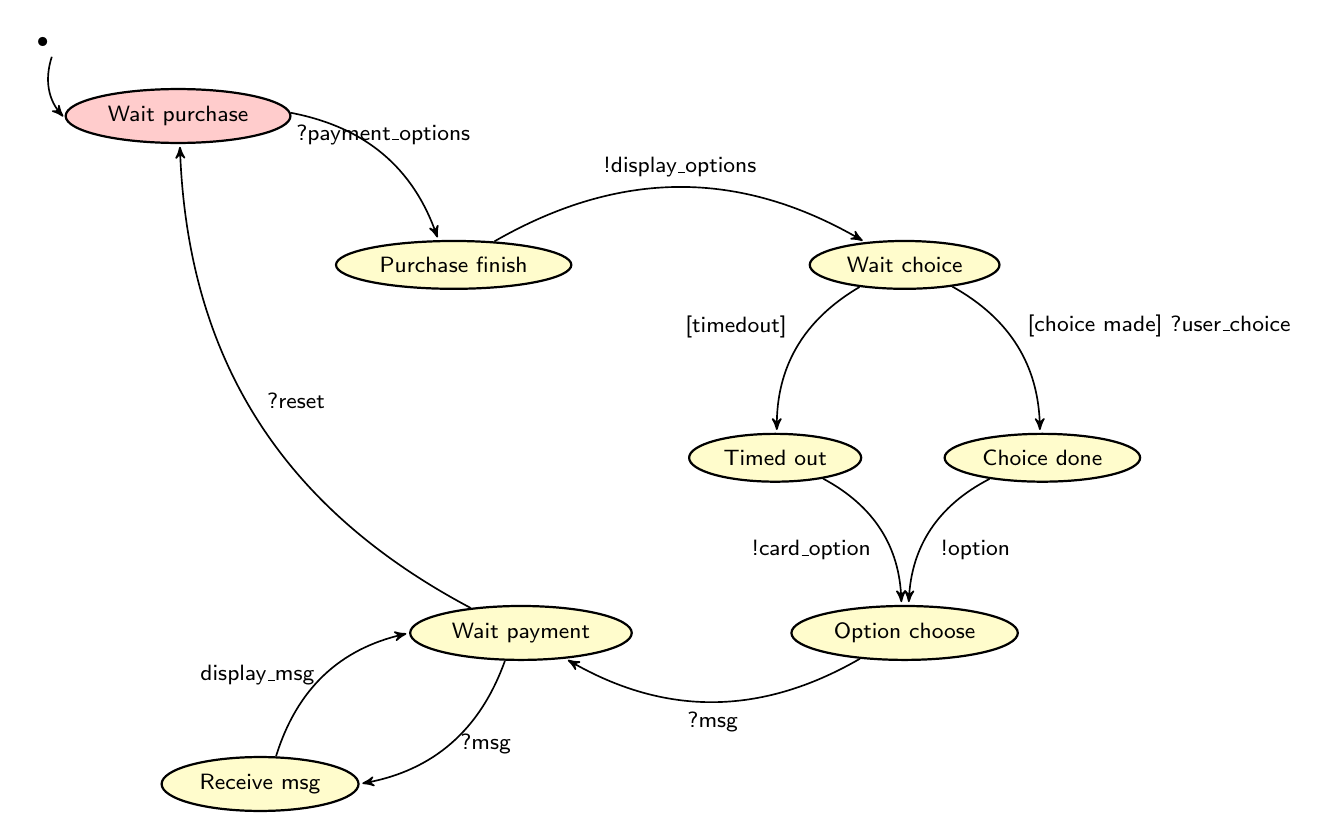
\begin{tikzpicture}[
            process/.style={draw,thick,ellipse,draw, minimum height=0.5cm, ellipse, fill=yellow!20},
            every node/.style={align=center, font=\sffamily\footnotesize},
            to/.style={->,>=stealth',shorten >=1pt,semithick,font=\sffamily\tiny},
            node distance = 2cm
  ]

  \node (start) {$\bullet$};
  \node[process, fill=red!20] (purchase) [below right=0.5cm and 0.5cm of start] {Wait purchase};
  \node[process] (finish) [below right=of purchase] {Purchase finish};
  \node[process] (display) [right=3cm of finish] {Wait choice};
  \node[process] (done) [below right=2cm and 0cm of display] {Choice done};
  \node[process] (timed) [below left=2cm and 0cm of display] {Timed out};
  \node[process] (choose) [below=4cm of display] {Option choose};
  \node[process] (paiment) [left=of choose] {Wait payment};
  \node[process] (msg) [below left=of paiment] {Receive msg};

  \draw[to] (purchase) edge[bend left] node[midway, above] {?payment\_options} (finish);
  \draw[to] (finish) edge[bend left] node[midway, above] {!display\_options} (display);

  \draw[to] (display) edge[bend left] node[midway, above right] {[choice made] ?user\_choice} (done);
  \draw[to] (display) edge[bend right] node[midway, above left] {[timedout]} (timed);
  \draw[to] (done) edge[bend right] node[midway, below right] {!option} (choose);
  \draw[to] (timed) edge[bend left] node[midway, below left] {!card\_option} (choose);

  \draw[to] (choose) edge[bend left] node[midway, below] {?msg} (paiment);

  \draw[to] (paiment) edge[bend left] node[midway, right] {?msg} (msg);
  \draw[to] (msg) edge[bend left] node[midway, left] {display\_msg} (paiment);

  \draw[to] (paiment) edge[bend left] node[midway, above right] {?reset} (purchase);

  \draw[to] (start) edge[bend right] (purchase);


\end{tikzpicture}
\caption{State diagram of gas pump interface}
\label{fig:state-gpi}
\end{figure}

\subsection{Cashier interface}

\begin{figure}[!h]
    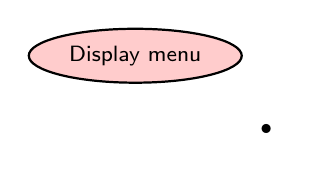
\begin{tikzpicture}[
            process/.style={draw,thick,ellipse,draw, minimum height=0.5cm, ellipse, fill=yellow!20},
            every node/.style={align=center, font=\sffamily\footnotesize},
            to/.style={->,>=stealth',shorten >=1pt,semithick,font=\sffamily\tiny},
            node distance = 2cm
  ]


  \node (start) {$\bullet$};
  \node[process, fill=red!20] (menu) [above left=0.5cm and 0.5cm of start] {Display menu};

\end{tikzpicture}
\caption{State diagram of cashier interface}
\label{fig:state-ci}
\end{figure}



\end{document}
